\documentclass[a4paper]{article}
\usepackage[a4paper]{geometry}
\usepackage{amsmath}
\usepackage{amssymb}
\usepackage[utf8]{inputenc}
\usepackage{graphicx}
\usepackage{booktabs}
\usepackage[russian]{babel}

\title{Лабораторная работа 1.3.3 \\Определение вязкости воздуха по скорости течения через тонкие трубки}
\date{20 февраля 2017 г.}
\author{Вячеслав Ждановский, студент 611 группы ФРКТ\\
Шамиль Вагабов, студент 611 группы ФРКТ\\
Станислав Токарев, студент 611 группы ФРКТ}

\begin{document}	\pagenumbering{gobble}
	\maketitle
	\newpage
	\pagenumbering{arabic}
	\paragraph{Цель работы:}
	экспериментально выявить участок сформированного течения, определить режимы ламинарного и турбулентного течения; определить число Рейнольдса.
	\paragraph{В работе используются:}
	металлические трубки, укрепленные на горизонтальной подставке; газовый счетчик; микроманометр типа ММН; стеклянная U-образная трубка; секундомер.
	\section{Теоретическая часть}
	Характер движения газа (или жидкости) в трубке определяется безразмерным числом Рейнольдса:
	\begin{equation}
	Re=\frac{\upsilon r\rho}{\eta}
	\end{equation}
	где $\upsilon$ - скорость потока, r - радиус трубки, $\rho$ - плотность движущейся среды, $\eta$ - её вязкость.
	При ламинарном течении объем газа V, протекающий за время t по трубе длиной l, определяется формулой Пуазёйля:
	\begin{equation}
	Q_v=\frac{\pi r^4}{8l\eta}(P_1-P_2)
	\end{equation}
	\section{Схема экспериментальной установки}
	\begin{figure}[h!]
		\centering
		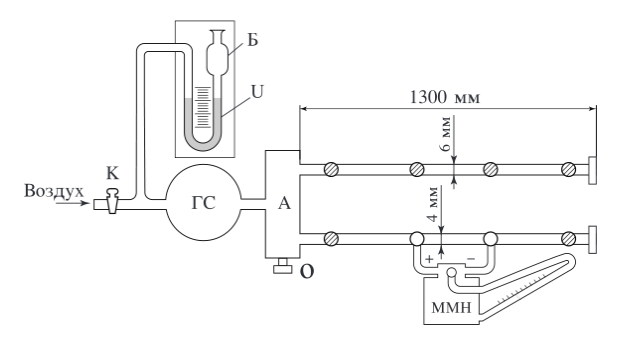
\includegraphics[width=70mm]{pic1.png}
		\caption{Схема экспериментальной установки \label{overflow}}
	\end{figure}
	\begin{figure}[h!]
		\centering
		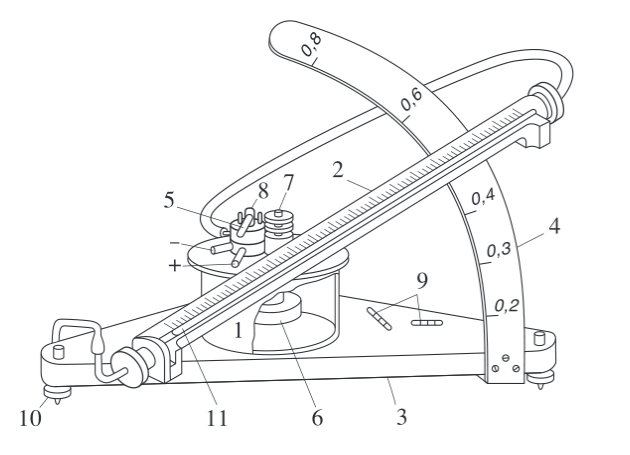
\includegraphics[width=70mm]{pic2.png}
		\caption{Микрометрический манометр типа ММН \label{overflow}}
	\end{figure}
	\begin{figure}[h!]
		\centering
		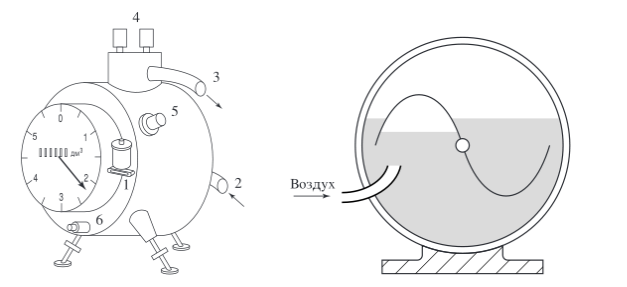
\includegraphics[width=70mm]{pic3.png}
		\caption{Внешний вид и схема устройства газового счетчика \label{overflow}}
	\end{figure}
	\newpage
	\section{Ход работы}
	\subsection{Оценим расстояние, на котором происходит формирование потока при ламинарном течении}
	\begin{equation}
		a\approx0,2r\cdot Re
	\end{equation}
	\paragraph{Трубка №1}
	\begin{equation}
		d=3,55\pm 0,05 \text{ мм}
	\end{equation}
	\begin{equation}
		r=\frac{d}{2}=1,78\pm 0,05 \text{ мм}
	\end{equation}
	\begin{equation}
		a\approx 0,2\cdot 1,78 \cdot 1000 \text{ мм}=356\text{ мм}\approx 0,35 \text{ м}
	\end{equation}
	\paragraph{Трубка №2}
	\begin{equation}
		d=5,00\pm 0,05 \text{ мм}
	\end{equation}
	\begin{equation}
		r=\frac{d}{2}=2,50\pm 0,05 \text{ мм}
	\end{equation}
	\begin{equation}
		a\approx 0,2\cdot 2,5 \cdot 1000 \text{ мм}=500\text{ мм}= 0,5 \text{ м}
	\end{equation}
	\paragraph{Трубка №3}
	\begin{equation}
		d=3,0\pm 0,1 \text{ мм}
	\end{equation}
	\begin{equation}
		r=\frac{d}{2}=1,5\pm 0,1 \text{ мм}
	\end{equation}
	\begin{equation}
		a\approx 0,2\cdot 1,5 \cdot 1000 \text{ мм}=300\text{ мм}= 0,3 \text{ м}
	\end{equation}
	\subsection{Заполним таблицу измерений}
	Медленно открывая кран, будем записывать показания микроманометра и газового счетчика. 
	\begin{equation}
	\Delta P=k\rho gh
	\end{equation}
	\begin{equation}
	\rho=0,8095 \text{ }\frac{\text{г}}{\text{см}^3}, \text{ } g=9,81 \text{ }\frac{\text{Н}}{\text{кг}}, \text{ }k=0,2
	\end{equation}
	\begin{table}[h!]
 		\centering
    	\begin{tabular}{|c|c|c|c|c|c|c|}
    		\hline
    		d, мм & h, мм & l, см & $\Delta$P, Па & $\Delta$V, дм$^3$ & t, c & Q, $\frac{\text{дм}^3}{\text{c}}$ \\
    		\hline
    		$3,55\pm0,05$ & 146 & 50 & 231 & 5 & 42 & 0,12 \\
    			& 236 & 50 & 375 & 4 & 29 & 0,14 \\
    		 	& 203 & 90 & 322 & 3 & 30 & 0,10 \\
    			& 265 & 90 & 420 & 7 & 61 & 0,11 \\
    			& 119 & 120 & 189 & 3 & 53 & 0,06 \\
    			& 217 & 120 & 345 & 5 & 55 & 0,10 \\
    			& 164 & 131 & 260 & 3 & 45.5 & 0,06 \\
    			& 245 & 131 & 389 & 2 & 24 & 0,08 \\
    		\hline
    		$5,00\pm0,05$ & 25 & 50 & 140 & 2 & 18 & 0,11 \\
    			& 65 & 50 & 103 & 2 & 12 & 0,17 \\
    		 	& 25 & 40 & 40 & 2 & 17 & 0,12 \\
    			& 50 & 40 & 80 & 2 & 16 & 0,125 \\
    			& 15 & 30 & 24 & 2 & 21 & 0,10 \\
    			& 35 & 30 & 56 & 2 & 12 & 0,17 \\
    			& 37 & 70 & 59 & 2 & 21 & 0,10 \\
    			& 74 & 70 & 118 & 2 & 13 & 0,15 \\
    			& 64 & 120 & 102 & 2 & 19 & 0,10 \\
    			& 170 & 120 & 270 & 2 & 12 & 0,17 \\
    		\hline
    		$3\pm0,1$ & 35 & 20 & ? & 2 & 22 & 0,10 \\
    			& 120 & 20 & 191 & 2 & 11 & 0,18 \\
    		 	& 30 & 26 & 48 & 2 & 50 & 0,04 \\
    			& 132 & 26 & 209 & 2 & 18 & 0,11 \\
    			& 28 & 46 & 44 & 2 & 66 & 0,03 \\
    			& 168 & 46 & 267 & 2 & 20 & 0,10 \\
    		\hline
    	\end{tabular}
  		\caption{Измерения зависимости $\Delta$P от Q}
	\end{table}
	\subsection{Найдем вязкость}
	\begin{equation}
	Q=\frac{\Delta V}{t}=\frac{\pi r^4}{8l\eta}\Delta P \rightarrow \eta = \frac{\pi r^4t\Delta P}{8l\Delta V}
	\end{equation}
	Вычислив и усреднив, получаем:
	\begin{equation}
	\eta = 16,3 \text{ Па}\cdot c
	\end{equation}
	\section{Графики}
	\begin{figure}[ht!]
		\centering
		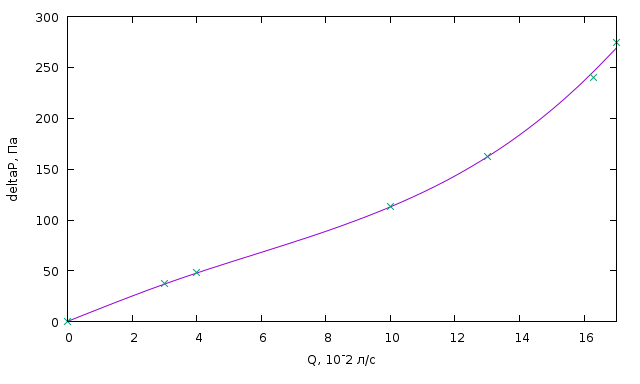
\includegraphics[width=125mm]{plot2.png}
		\caption{Зависимость $\Delta$P от Q\label{overflow}}
	\end{figure}
	\begin{figure}[ht!]
		\centering
		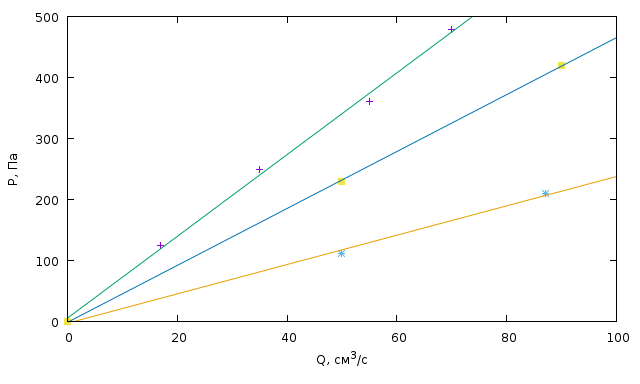
\includegraphics[width=125mm]{plot1.png}
		\caption{Зависимость P от Q\label{overflow}}
	\end{figure}
\end{document}